\section{Glossario e Class Diagram}

\subsection{Class Diagram}
Il diagramma seguente rappresenta le entità di dominio e le relative
relazioni cardinali.

\begin{figure}[H]
    \centering
    % 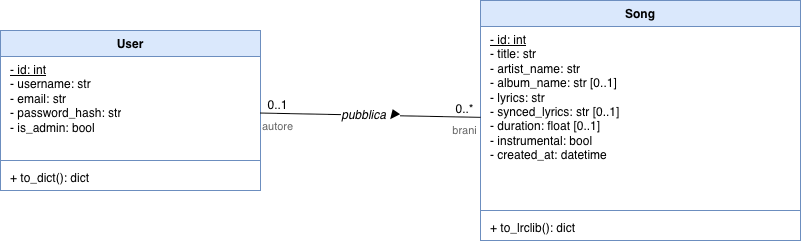
\includegraphics[width=\textwidth]{class-diagram.png}
    \fbox{\parbox{0.85\textwidth}{\centering\vspace{1em}
        \TODO{Inserire il \emph{Class Diagram} UML che rappresenta le
        classi: \code{User}, \code{Artist}, \code{Album}, \code{Song},
        \code{PowChallenge}, con relazioni cardinali (es. Artist 1..* Song,
        Album 0..1 -- 0..* Song, User 0..1 -- 0..* Song).}
        \vspace{1em}}}
    \caption{Class Diagram di Stopify.}
    \label{fig:classdiagram}
\end{figure}

\subsection{Glossario dei termini}
\begin{table}[H]
    \centering
    \begin{tabularx}{\textwidth}{@{}lX@{}}
        \toprule
        \textbf{Termine} & \textbf{Descrizione} \\
        \midrule
        Lyric / Testo &
        Insieme delle parole cantate in un brano musicale. Memorizzato in
        forma piana (\code{plainLyrics}) e/o sincronizzata
        (\code{syncedLyrics}). \\

        Plain lyrics &
        Testo in chiaro privo di marcatori temporali, suddiviso in righe e
        strofe. \\

        Synced lyrics (LRC) &
        Testo con timestamp del tipo \code{[mm:ss.xx]} che indicano il
        momento esatto in cui ogni riga viene cantata. Formato standard
        \emph{LRC}. \\

        LRCLIB &
        Servizio open di lyrics il cui schema API è emulato dal nostro
        backend. \\

        Signature di un brano &
        Tupla (titolo, artista, eventualmente album, durata) usata per
        identificare univocamente un brano nelle query LRCLIB. \\

        Track / Brano (\code{Song}) &
        Entità che rappresenta un singolo brano con titolo, testo, riferimento
        all'artista, opzionalmente album e utente che lo ha pubblicato. \\

        Artist &
        Entità che rappresenta un artista o un gruppo musicale. \\

        Album &
        Entità opzionale che raggruppa più brani dello stesso artista. \\

        User &
        Utente registrato; possiede credenziali (username, email, password
        hashata) e può pubblicare brani attribuiti. \\

        JWT &
        \emph{JSON Web Token}: stringa firmata che porta l'identità
        dell'utente. Inviato dal client nell'header \code{Authorization} per
        autenticare le richieste. \\

        Access token &
        JWT a breve durata usato per autenticare le chiamate API.
        Inviato nell'header \code{Authorization: Bearer <token>}.
        Alla scadenza l'utente deve effettuare nuovamente il login. \\

        Proof of Work (PoW) &
        Sfida crittografica che il client deve risolvere via brute force
        prima di poter inviare una pubblicazione anonima. Disincentiva lo
        spam massivo. \\

        \code{submittedBy} &
        Campo della risposta che indica lo username dell'autore di un
        brano (\code{null} se anonimo). \\

        ORM &
        \emph{Object-Relational Mapping}: mappatura tra classi Python e
        tabelle del DB realizzata tramite SQLAlchemy. \\

        CORS &
        \emph{Cross-Origin Resource Sharing}: meccanismo del browser che
        regola le richieste cross-origin verso il backend. \\

        \bottomrule
    \end{tabularx}
    \caption{Glossario.}
\end{table}
